% Created by tikzDevice version 0.12.3.1 on 2022-02-03 17:36:37
% !TEX encoding = UTF-8 Unicode
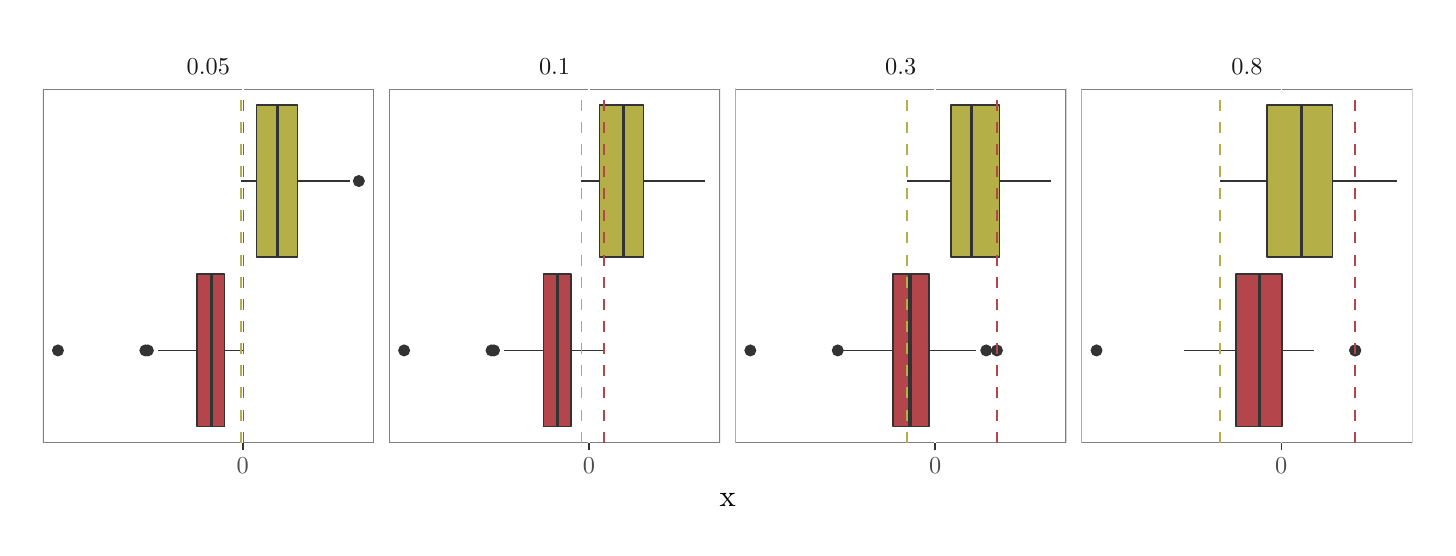
\begin{tikzpicture}[x=1pt,y=1pt]
\definecolor{fillColor}{RGB}{255,255,255}
\path[use as bounding box,fill=fillColor,fill opacity=0.00] (0,0) rectangle (505.89,180.67);
\begin{scope}
\path[clip] (  0.00,  0.00) rectangle (505.89,180.67);
\definecolor{drawColor}{RGB}{255,255,255}
\definecolor{fillColor}{RGB}{255,255,255}

\path[draw=drawColor,line width= 0.6pt,line join=round,line cap=round,fill=fillColor] (  0.00,  0.00) rectangle (505.89,180.68);
\end{scope}
\begin{scope}
\path[clip] (  5.50, 30.69) rectangle (125.10,158.60);
\definecolor{drawColor}{gray}{0.50}
\definecolor{fillColor}{RGB}{255,255,255}

\path[draw=drawColor,line width= 0.6pt,line join=round,line cap=round,fill=fillColor] (  5.50, 30.69) rectangle (125.10,158.60);
\definecolor{drawColor}{RGB}{255,255,255}

\path[draw=drawColor,line width= 0.6pt,line join=round] ( 77.71, 30.69) --
	( 77.71,158.60);
\definecolor{drawColor}{gray}{0.20}
\definecolor{fillColor}{gray}{0.20}

\path[draw=drawColor,line width= 0.4pt,line join=round,line cap=round,fill=fillColor] ( 43.42, 64.04) circle (  1.96);

\path[draw=drawColor,line width= 0.4pt,line join=round,line cap=round,fill=fillColor] ( 10.94, 64.04) circle (  1.96);

\path[draw=drawColor,line width= 0.4pt,line join=round,line cap=round,fill=fillColor] ( 42.52, 64.04) circle (  1.96);

\path[draw=drawColor,line width= 0.6pt,line join=round] ( 71.16, 64.04) -- ( 78.04, 64.04);

\path[draw=drawColor,line width= 0.6pt,line join=round] ( 61.29, 64.04) -- ( 47.15, 64.04);
\definecolor{fillColor}{RGB}{180,70,75}

\path[draw=drawColor,line width= 0.6pt,line join=round,line cap=round,fill=fillColor] ( 71.16, 36.50) --
	( 61.29, 36.50) --
	( 61.29, 91.58) --
	( 71.16, 91.58) --
	( 71.16, 36.50) --
	cycle;

\path[draw=drawColor,line width= 1.1pt,line join=round] ( 66.42, 36.50) -- ( 66.42, 91.58);
\definecolor{fillColor}{gray}{0.20}

\path[draw=drawColor,line width= 0.4pt,line join=round,line cap=round,fill=fillColor] (119.66,125.25) circle (  1.96);

\path[draw=drawColor,line width= 0.6pt,line join=round] ( 97.46,125.25) -- (116.37,125.25);

\path[draw=drawColor,line width= 0.6pt,line join=round] ( 82.67,125.25) -- ( 77.08,125.25);
\definecolor{fillColor}{RGB}{180,175,70}

\path[draw=drawColor,line width= 0.6pt,line join=round,line cap=round,fill=fillColor] ( 97.46, 97.70) --
	( 82.67, 97.70) --
	( 82.67,152.79) --
	( 97.46,152.79) --
	( 97.46, 97.70) --
	cycle;

\path[draw=drawColor,line width= 1.1pt,line join=round] ( 90.23, 97.70) -- ( 90.23,152.79);
\definecolor{drawColor}{RGB}{180,175,70}

\path[draw=drawColor,line width= 0.6pt,dash pattern=on 4pt off 4pt ,line join=round] ( 77.08, 30.69) -- ( 77.08,158.60);
\definecolor{drawColor}{RGB}{180,70,75}

\path[draw=drawColor,line width= 0.6pt,dash pattern=on 4pt off 4pt ,line join=round] ( 78.04, 30.69) -- ( 78.04,158.60);
\end{scope}
\begin{scope}
\path[clip] (130.60, 30.69) rectangle (250.19,158.60);
\definecolor{drawColor}{gray}{0.50}
\definecolor{fillColor}{RGB}{255,255,255}

\path[draw=drawColor,line width= 0.6pt,line join=round,line cap=round,fill=fillColor] (130.60, 30.69) rectangle (250.19,158.60);
\definecolor{drawColor}{RGB}{255,255,255}

\path[draw=drawColor,line width= 0.6pt,line join=round] (202.81, 30.69) --
	(202.81,158.60);
\definecolor{drawColor}{gray}{0.20}
\definecolor{fillColor}{gray}{0.20}

\path[draw=drawColor,line width= 0.4pt,line join=round,line cap=round,fill=fillColor] (168.51, 64.04) circle (  1.96);

\path[draw=drawColor,line width= 0.4pt,line join=round,line cap=round,fill=fillColor] (136.03, 64.04) circle (  1.96);

\path[draw=drawColor,line width= 0.4pt,line join=round,line cap=round,fill=fillColor] (167.61, 64.04) circle (  1.96);

\path[draw=drawColor,line width= 0.6pt,line join=round] (196.26, 64.04) -- (208.35, 64.04);

\path[draw=drawColor,line width= 0.6pt,line join=round] (186.39, 64.04) -- (172.24, 64.04);
\definecolor{fillColor}{RGB}{180,70,75}

\path[draw=drawColor,line width= 0.6pt,line join=round,line cap=round,fill=fillColor] (196.26, 36.50) --
	(186.39, 36.50) --
	(186.39, 91.58) --
	(196.26, 91.58) --
	(196.26, 36.50) --
	cycle;

\path[draw=drawColor,line width= 1.1pt,line join=round] (191.52, 36.50) -- (191.52, 91.58);

\path[draw=drawColor,line width= 0.6pt,line join=round] (222.55,125.25) -- (244.76,125.25);

\path[draw=drawColor,line width= 0.6pt,line join=round] (206.61,125.25) -- (200.09,125.25);
\definecolor{fillColor}{RGB}{180,175,70}

\path[draw=drawColor,line width= 0.6pt,line join=round,line cap=round,fill=fillColor] (222.55, 97.70) --
	(206.61, 97.70) --
	(206.61,152.79) --
	(222.55,152.79) --
	(222.55, 97.70) --
	cycle;

\path[draw=drawColor,line width= 1.1pt,line join=round] (215.33, 97.70) -- (215.33,152.79);
\definecolor{drawColor}{RGB}{180,175,70}

\path[draw=drawColor,line width= 0.6pt,dash pattern=on 4pt off 4pt ,line join=round] (200.09, 30.69) -- (200.09,158.60);
\definecolor{drawColor}{RGB}{180,70,75}

\path[draw=drawColor,line width= 0.6pt,dash pattern=on 4pt off 4pt ,line join=round] (208.35, 30.69) -- (208.35,158.60);
\end{scope}
\begin{scope}
\path[clip] (255.69, 30.69) rectangle (375.29,158.60);
\definecolor{drawColor}{gray}{0.50}
\definecolor{fillColor}{RGB}{255,255,255}

\path[draw=drawColor,line width= 0.6pt,line join=round,line cap=round,fill=fillColor] (255.70, 30.69) rectangle (375.29,158.60);
\definecolor{drawColor}{RGB}{255,255,255}

\path[draw=drawColor,line width= 0.6pt,line join=round] (327.91, 30.69) --
	(327.91,158.60);
\definecolor{drawColor}{gray}{0.20}
\definecolor{fillColor}{gray}{0.20}

\path[draw=drawColor,line width= 0.4pt,line join=round,line cap=round,fill=fillColor] (261.13, 64.04) circle (  1.96);

\path[draw=drawColor,line width= 0.4pt,line join=round,line cap=round,fill=fillColor] (350.24, 64.04) circle (  1.96);

\path[draw=drawColor,line width= 0.4pt,line join=round,line cap=round,fill=fillColor] (292.71, 64.04) circle (  1.96);

\path[draw=drawColor,line width= 0.4pt,line join=round,line cap=round,fill=fillColor] (346.37, 64.04) circle (  1.96);

\path[draw=drawColor,line width= 0.6pt,line join=round] (325.70, 64.04) -- (342.77, 64.04);

\path[draw=drawColor,line width= 0.6pt,line join=round] (312.57, 64.04) -- (293.61, 64.04);
\definecolor{fillColor}{RGB}{180,70,75}

\path[draw=drawColor,line width= 0.6pt,line join=round,line cap=round,fill=fillColor] (325.70, 36.50) --
	(312.57, 36.50) --
	(312.57, 91.58) --
	(325.70, 91.58) --
	(325.70, 36.50) --
	cycle;

\path[draw=drawColor,line width= 1.1pt,line join=round] (318.83, 36.50) -- (318.83, 91.58);

\path[draw=drawColor,line width= 0.6pt,line join=round] (351.17,125.25) -- (369.86,125.25);

\path[draw=drawColor,line width= 0.6pt,line join=round] (333.72,125.25) -- (317.78,125.25);
\definecolor{fillColor}{RGB}{180,175,70}

\path[draw=drawColor,line width= 0.6pt,line join=round,line cap=round,fill=fillColor] (351.17, 97.70) --
	(333.72, 97.70) --
	(333.72,152.79) --
	(351.17,152.79) --
	(351.17, 97.70) --
	cycle;

\path[draw=drawColor,line width= 1.1pt,line join=round] (340.94, 97.70) -- (340.94,152.79);
\definecolor{drawColor}{RGB}{180,175,70}

\path[draw=drawColor,line width= 0.6pt,dash pattern=on 4pt off 4pt ,line join=round] (317.78, 30.69) -- (317.78,158.60);
\definecolor{drawColor}{RGB}{180,70,75}

\path[draw=drawColor,line width= 0.6pt,dash pattern=on 4pt off 4pt ,line join=round] (350.24, 30.69) -- (350.24,158.60);
\end{scope}
\begin{scope}
\path[clip] (380.79, 30.69) rectangle (500.39,158.60);
\definecolor{drawColor}{gray}{0.50}
\definecolor{fillColor}{RGB}{255,255,255}

\path[draw=drawColor,line width= 0.6pt,line join=round,line cap=round,fill=fillColor] (380.79, 30.69) rectangle (500.39,158.60);
\definecolor{drawColor}{RGB}{255,255,255}

\path[draw=drawColor,line width= 0.6pt,line join=round] (453.01, 30.69) --
	(453.01,158.60);
\definecolor{drawColor}{gray}{0.20}
\definecolor{fillColor}{gray}{0.20}

\path[draw=drawColor,line width= 0.4pt,line join=round,line cap=round,fill=fillColor] (386.23, 64.04) circle (  1.96);

\path[draw=drawColor,line width= 0.4pt,line join=round,line cap=round,fill=fillColor] (479.65, 64.04) circle (  1.96);

\path[draw=drawColor,line width= 0.4pt,line join=round,line cap=round,fill=fillColor] (479.73, 64.04) circle (  1.96);

\path[draw=drawColor,line width= 0.6pt,line join=round] (453.14, 64.04) -- (464.67, 64.04);

\path[draw=drawColor,line width= 0.6pt,line join=round] (436.59, 64.04) -- (417.81, 64.04);
\definecolor{fillColor}{RGB}{180,70,75}

\path[draw=drawColor,line width= 0.6pt,line join=round,line cap=round,fill=fillColor] (453.14, 36.50) --
	(436.59, 36.50) --
	(436.59, 91.58) --
	(453.14, 91.58) --
	(453.14, 36.50) --
	cycle;

\path[draw=drawColor,line width= 1.1pt,line join=round] (445.17, 36.50) -- (445.17, 91.58);

\path[draw=drawColor,line width= 0.6pt,line join=round] (471.52,125.25) -- (494.95,125.25);

\path[draw=drawColor,line width= 0.6pt,line join=round] (447.90,125.25) -- (430.88,125.25);
\definecolor{fillColor}{RGB}{180,175,70}

\path[draw=drawColor,line width= 0.6pt,line join=round,line cap=round,fill=fillColor] (471.52, 97.70) --
	(447.90, 97.70) --
	(447.90,152.79) --
	(471.52,152.79) --
	(471.52, 97.70) --
	cycle;

\path[draw=drawColor,line width= 1.1pt,line join=round] (460.17, 97.70) -- (460.17,152.79);
\definecolor{drawColor}{RGB}{180,175,70}

\path[draw=drawColor,line width= 0.6pt,dash pattern=on 4pt off 4pt ,line join=round] (430.88, 30.69) -- (430.88,158.60);
\definecolor{drawColor}{RGB}{180,70,75}

\path[draw=drawColor,line width= 0.6pt,dash pattern=on 4pt off 4pt ,line join=round] (479.73, 30.69) -- (479.73,158.60);
\end{scope}
\begin{scope}
\path[clip] (  5.50,158.60) rectangle (125.10,175.17);
\definecolor{fillColor}{RGB}{255,255,255}

\path[fill=fillColor] (  5.50,158.60) rectangle (125.10,175.18);
\definecolor{drawColor}{gray}{0.10}

\node[text=drawColor,anchor=base,inner sep=0pt, outer sep=0pt, scale=  0.88] at ( 65.30,163.86) {0.05};
\end{scope}
\begin{scope}
\path[clip] (130.60,158.60) rectangle (250.19,175.17);
\definecolor{fillColor}{RGB}{255,255,255}

\path[fill=fillColor] (130.60,158.60) rectangle (250.19,175.18);
\definecolor{drawColor}{gray}{0.10}

\node[text=drawColor,anchor=base,inner sep=0pt, outer sep=0pt, scale=  0.88] at (190.40,163.86) {0.1};
\end{scope}
\begin{scope}
\path[clip] (255.69,158.60) rectangle (375.29,175.17);
\definecolor{fillColor}{RGB}{255,255,255}

\path[fill=fillColor] (255.70,158.60) rectangle (375.29,175.18);
\definecolor{drawColor}{gray}{0.10}

\node[text=drawColor,anchor=base,inner sep=0pt, outer sep=0pt, scale=  0.88] at (315.49,163.86) {0.3};
\end{scope}
\begin{scope}
\path[clip] (380.79,158.60) rectangle (500.39,175.17);
\definecolor{fillColor}{RGB}{255,255,255}

\path[fill=fillColor] (380.79,158.60) rectangle (500.39,175.18);
\definecolor{drawColor}{gray}{0.10}

\node[text=drawColor,anchor=base,inner sep=0pt, outer sep=0pt, scale=  0.88] at (440.59,163.86) {0.8};
\end{scope}
\begin{scope}
\path[clip] (  0.00,  0.00) rectangle (505.89,180.67);
\definecolor{drawColor}{gray}{0.20}

\path[draw=drawColor,line width= 0.6pt,line join=round] ( 77.71, 27.94) --
	( 77.71, 30.69);
\end{scope}
\begin{scope}
\path[clip] (  0.00,  0.00) rectangle (505.89,180.67);
\definecolor{drawColor}{gray}{0.30}

\node[text=drawColor,anchor=base,inner sep=0pt, outer sep=0pt, scale=  0.88] at ( 77.71, 19.68) {0};
\end{scope}
\begin{scope}
\path[clip] (  0.00,  0.00) rectangle (505.89,180.67);
\definecolor{drawColor}{gray}{0.20}

\path[draw=drawColor,line width= 0.6pt,line join=round] (202.81, 27.94) --
	(202.81, 30.69);
\end{scope}
\begin{scope}
\path[clip] (  0.00,  0.00) rectangle (505.89,180.67);
\definecolor{drawColor}{gray}{0.30}

\node[text=drawColor,anchor=base,inner sep=0pt, outer sep=0pt, scale=  0.88] at (202.81, 19.68) {0};
\end{scope}
\begin{scope}
\path[clip] (  0.00,  0.00) rectangle (505.89,180.67);
\definecolor{drawColor}{gray}{0.20}

\path[draw=drawColor,line width= 0.6pt,line join=round] (327.91, 27.94) --
	(327.91, 30.69);
\end{scope}
\begin{scope}
\path[clip] (  0.00,  0.00) rectangle (505.89,180.67);
\definecolor{drawColor}{gray}{0.30}

\node[text=drawColor,anchor=base,inner sep=0pt, outer sep=0pt, scale=  0.88] at (327.91, 19.68) {0};
\end{scope}
\begin{scope}
\path[clip] (  0.00,  0.00) rectangle (505.89,180.67);
\definecolor{drawColor}{gray}{0.20}

\path[draw=drawColor,line width= 0.6pt,line join=round] (453.01, 27.94) --
	(453.01, 30.69);
\end{scope}
\begin{scope}
\path[clip] (  0.00,  0.00) rectangle (505.89,180.67);
\definecolor{drawColor}{gray}{0.30}

\node[text=drawColor,anchor=base,inner sep=0pt, outer sep=0pt, scale=  0.88] at (453.01, 19.68) {0};
\end{scope}
\begin{scope}
\path[clip] (  0.00,  0.00) rectangle (505.89,180.67);
\definecolor{drawColor}{RGB}{0,0,0}

\node[text=drawColor,anchor=base,inner sep=0pt, outer sep=0pt, scale=  1.10] at (252.94,  7.64) {x};
\end{scope}
\end{tikzpicture}
